\chapter{Experimental setup and tests on board}
\section{Introduction}
In section \ref{hardware} will be described a simple level translator built for simulation purposes while in sections \ref{testbench} and \ref{testboard} will be briefly analyzed the experimental setup.

\section{Test Bench}\label{testbench}
\begin{figure}[H]
	\centering
	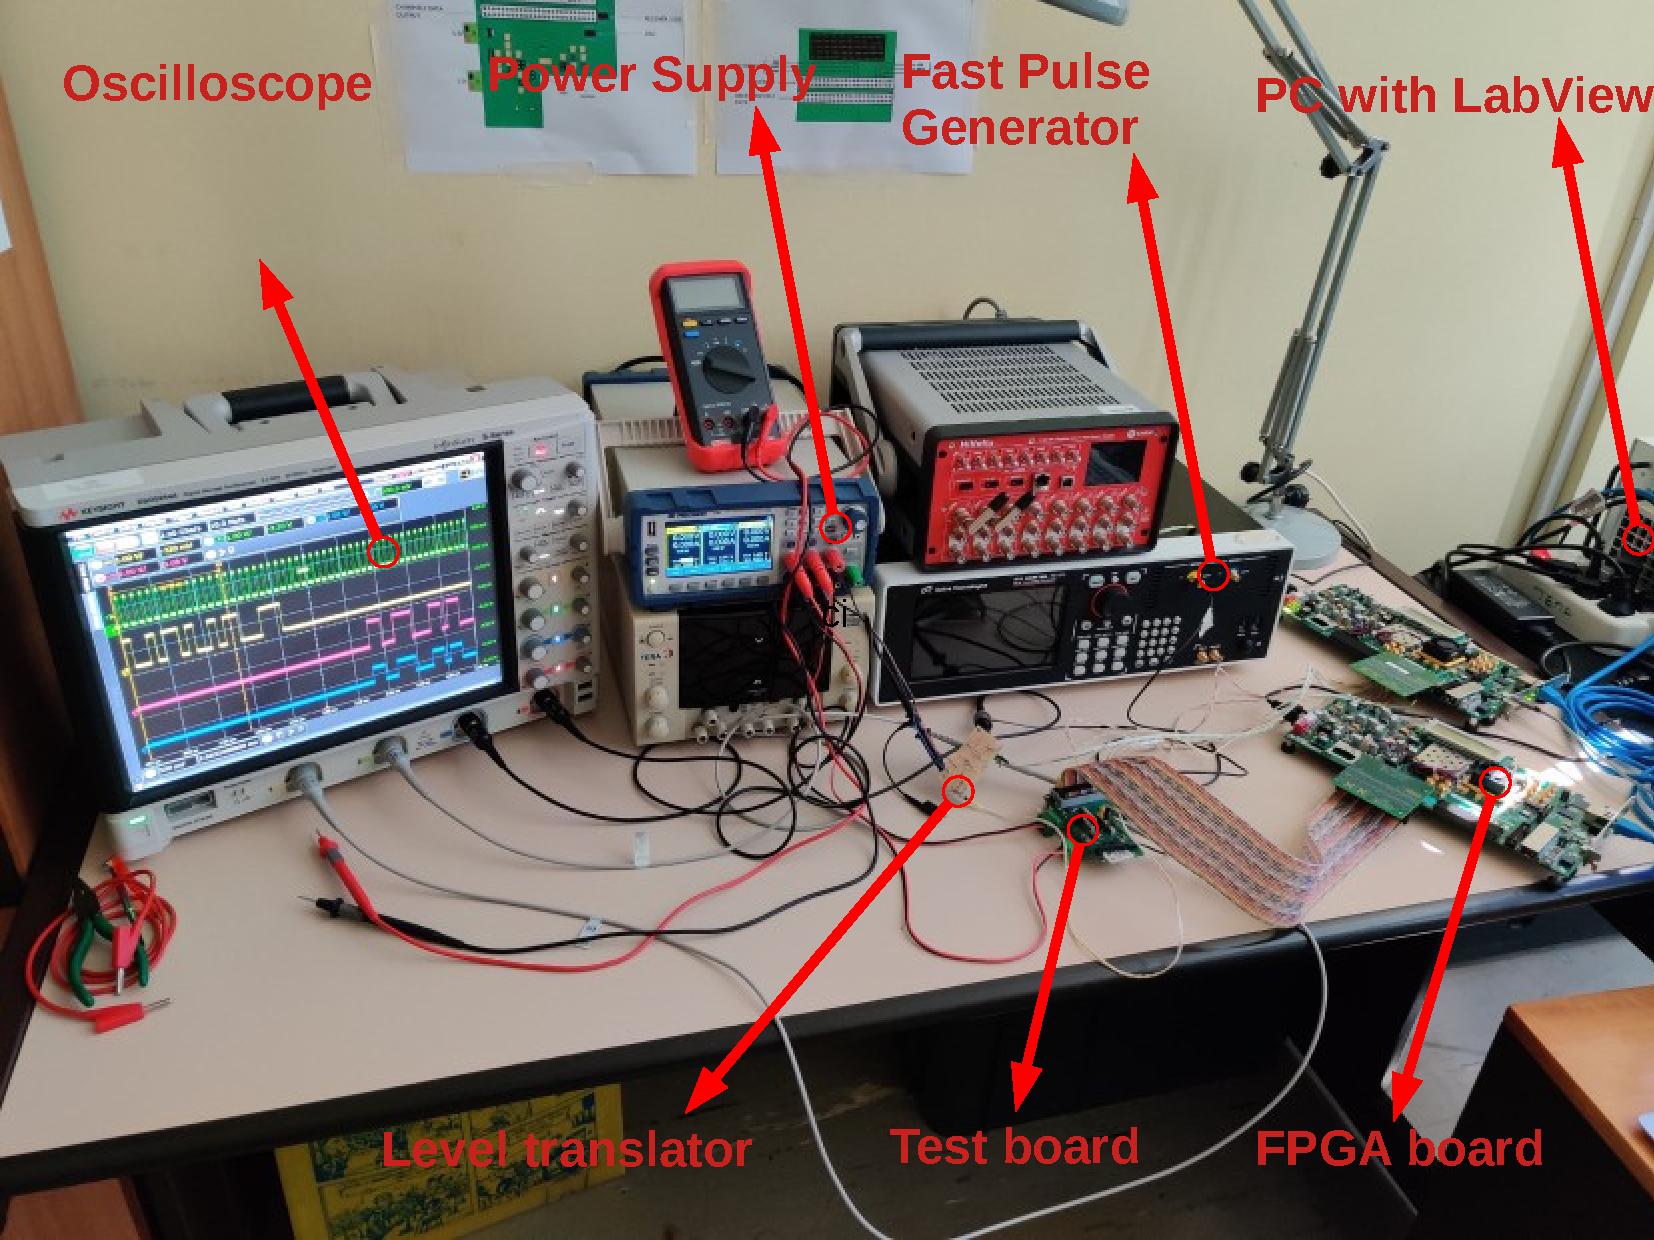
\includegraphics[width=0.7\linewidth]{IMG/ch5/TESTBENCH}
	\caption{Test bench setup and devices}
	\label{fig:testbench}
\end{figure}
In order to properly validate the new additions of the FPGA firmware, after the simulations performed in the Vivado design suite, numerous tests have been carried out on the FPGA board and on chip.
The setup used to perform the test is shown in figure \ref{fig:testbench} and it comprehends:
\begin{itemize}
	\item A keysight DSOS254A (Digital Storage Oscilloscope), 4-channels, 2.5~GHz, 20~GSa/s, 10~bit ADC professional oscilloscope
	\item A power supply for the test board and the level translator
	\item A Fast Pulse Generator used to simulate the signal coming from the detector
	\item A computer with LabView
	\item The FPGA board with the NEW firmware that needs to be tested
	\item The test board with the ABACUS\_v2 bonded to it
	\item A level translator device that will be explained better in section \ref{hardware}
\end{itemize}

\section{Test board}\label{testboard}
\begin{figure}[H]
	\centering
	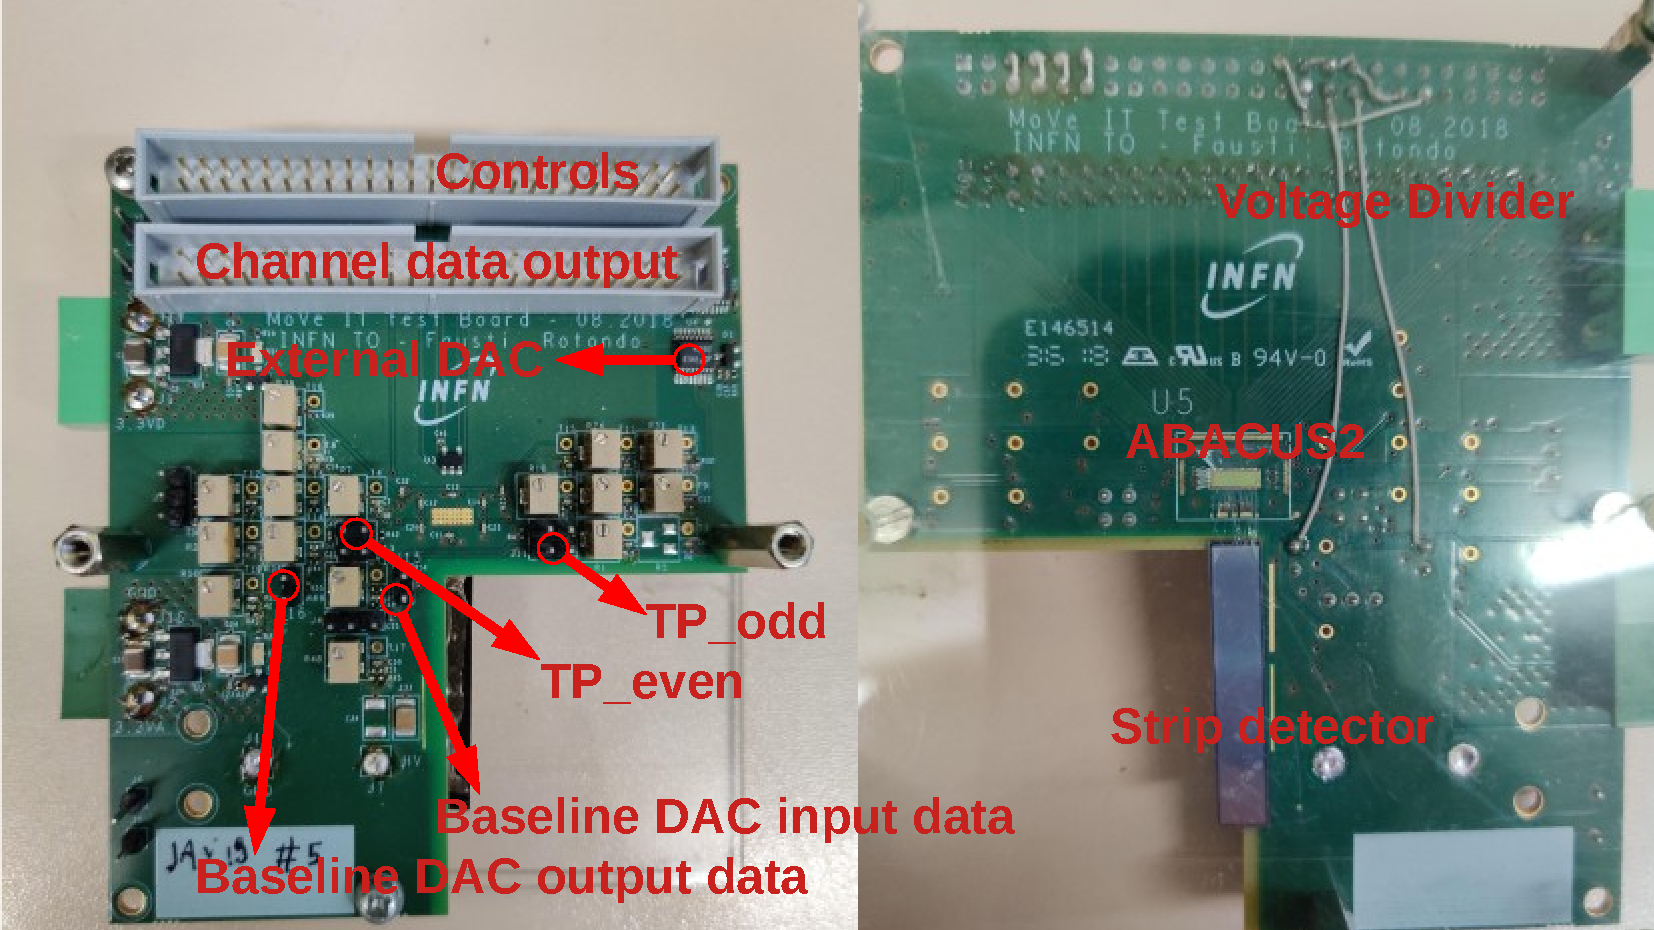
\includegraphics[width=0.7\linewidth]{IMG/ch5/TESTBOARD}
	\caption{Test board top and bottom view}
	\label{fig:testboard}
\end{figure}
To test every feature of the ABACUS\_v2 chip the INFN Turin section projected and created a test board.
On the back side of the PCB, shown in figure \ref{fig:testboard}, it can be observed the naked chip bonded to the board.
Moreover, the main components of the test board are:
\begin{itemize}
	\item Two 50 pin connectors, the bottom one is used to send the bipolar data from the chip to the FPGA and the top one is used to receive the controls (main DAC, trimming DACs, clocks) to the board
	\begin{figure}[H]
		\centering
		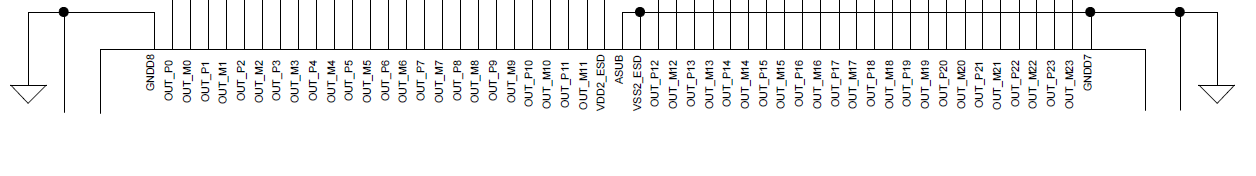
\includegraphics[width=0.95\linewidth]{IMG/ch5/DATATOFPGA}
		\caption{Wiring from the chip to the bottom 50 PIN connector}
		\label{fig:datatofpga}
	\end{figure}
	\item The external DAC, a commercially available Linear Technology LTC2604 \cite{LTC2604} Quad 16-bit Rail-to-Rail DAC, connected as in figure \ref{fig:externaldac}
	\begin{figure}[H]
		\centering
		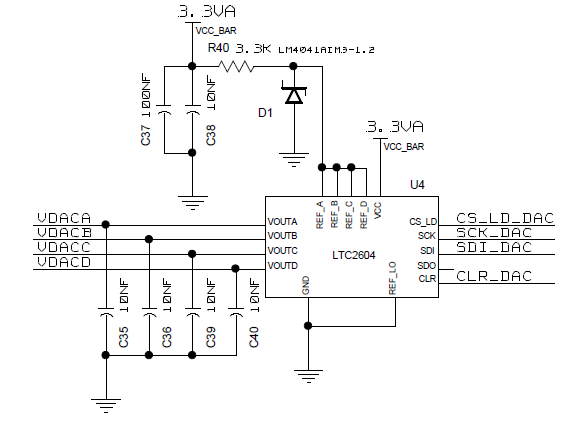
\includegraphics[width=0.3\linewidth]{IMG/ch5/EXTERNALDAC}
		\caption{Connections of the LTC2604 external DAC}
		\label{fig:externaldac}
	\end{figure}
	\item Two TP (Test Pulse) connectors (\textit{TP\_odd} and \textit{TP\_even}) used to inject a charge and thus simulate the signal from the LGAD detector, connected to the chip as in figure \ref{fig:tpconnector}
	\begin{figure}[H]
		\centering
		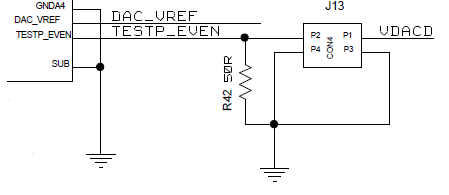
\includegraphics[width=0.4\linewidth]{IMG/ch5/TPCONNECTOR}
		\caption{Wiring of the \textit{TP\_even} connector}
		\label{fig:tpconnector}
	\end{figure}
	\item Two connectors (Baseline DAC input data and Baseline DAC output data) used to send and receive data from the internal DACs, wired as in figure \ref{fig:internaldacwiring} with a 50~$\Omega$ termination 
	\begin{figure}[H]
		\centering
		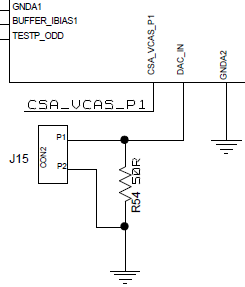
\includegraphics[width=0.2\linewidth]{IMG/ch5/INTERNALDACWIRING}
		\caption{Wiring of the Baseline (trimming/internal) DAC data in connector}
		\label{fig:internaldacwiring}
	\end{figure} 
\end{itemize} 
\noindent The 50 PIN connector is connected to the FMC port by means of a breakout board that can be seen attached to the FPGA in figure \ref{fig:testbench}. This PCB has no electrical components, only wiring to adapt one physical connector to another.
\section{Hardware devices}\label{hardware}
\noindent As described previously the ABACUS\_v2 chip, for the configuration and readout of the internal DACs, works on 1,2~V LVCMOS single-ended signal only. however the FPGA uses only one reference voltage for the entire FMC connector, this means that for how the board is configured it is impossible to send and receive 1,2~V signals.
In order to solve this problem two simple devices have been implemented; a voltage divider and a level translator device.
\subsubsection{Voltage divider}
On the one hand the data coming from the FPGA to the chip is at 2,5~V single-ended. To lower this value it has been implemented a simple voltage divider with 2 SMD (Surface-Mount Devices) resistors
\subsubsection{Level translator}
On the other hand the data coming from the chip is at 1.2~V. This value is too low and thus the board reads it always as \textit{low}. A voltage translation device is needed in order to boost the signal \textit{high} value. For this purpose I created the simple circuit in figure \ref{fig:diagram} using three 1~k$\Omega$ resistor and two classic \textit{2N2222} transistors that are configured in the standard common emitter mode.
\begin{figure}[H]
	\centering
	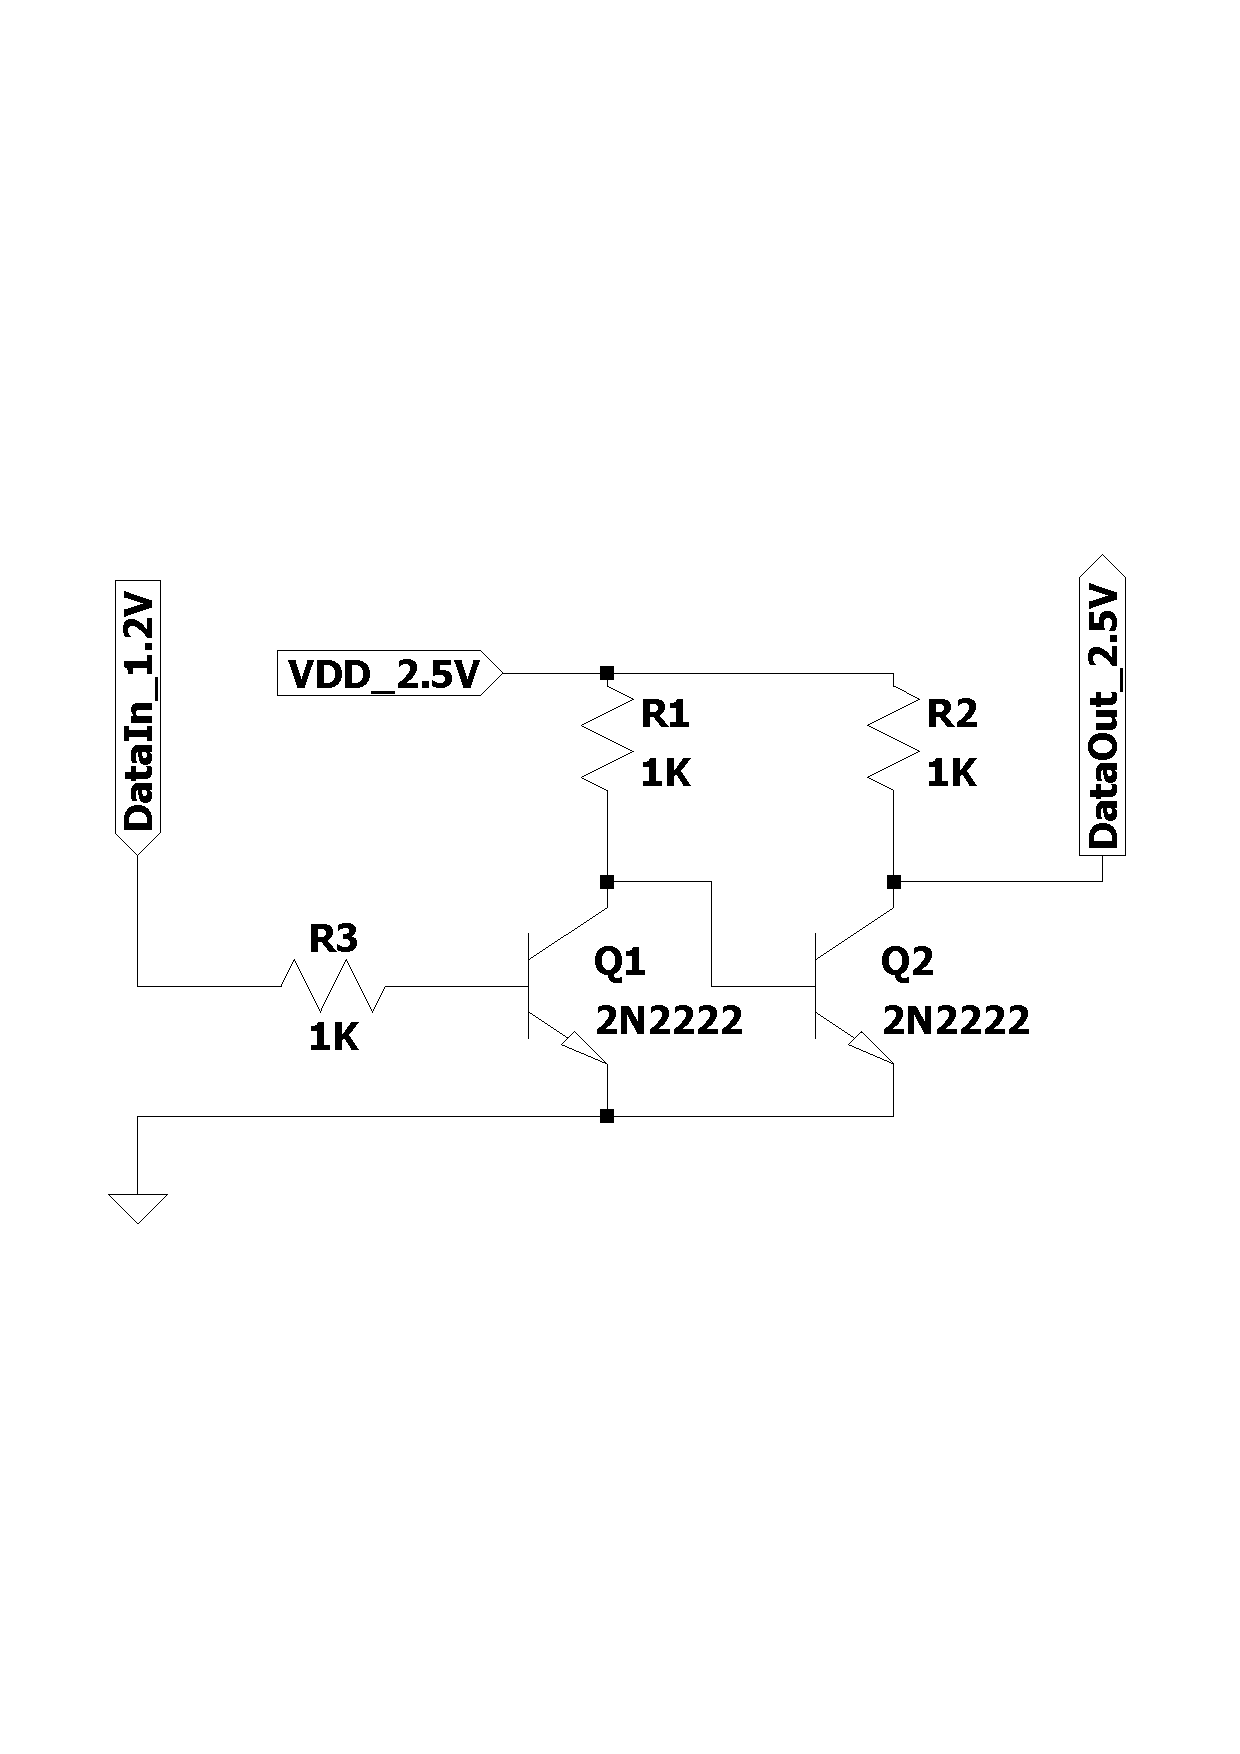
\includegraphics[width=0.5\linewidth]{IMG/ch5/DIAGRAM}
	\caption{Diagram of the level translation device}
	\label{fig:diagram}
\end{figure}
\noindent This device has been simulated using LTspice simulator and the results can be seen in figure \ref{fig:transsimulation}. The green signal is the input data at 1.2~V while the purple one is the output signal at 2.5~V.
According to the simulation the device works properly and thus it can be implemented in hardware.
\begin{figure}[H]
	\centering
	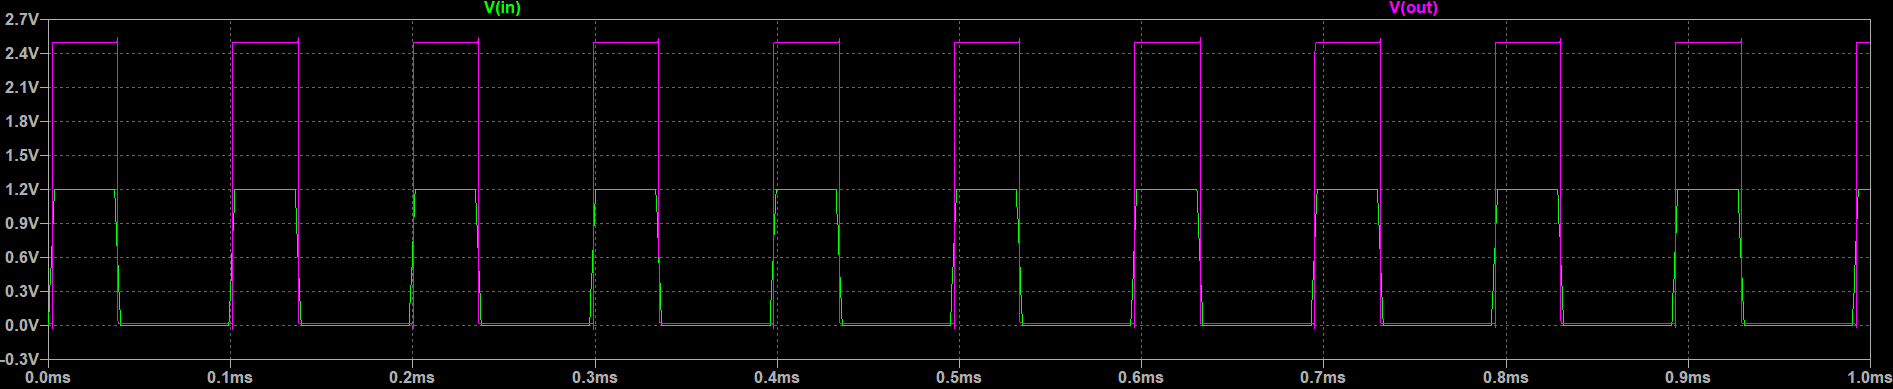
\includegraphics[width=1\linewidth]{IMG/ch5/TRANSSIMULATION}
	\caption{LTspice simulation of the translation device}
	\label{fig:transsimulation}
\end{figure}
\noindent The device was built soldering the components on a piece of perfboard that can be seen in figure \ref{fig:fronttranslator} and \ref{fig:backtranslator}.
\begin{figure}[H]
	\centering
	\begin{minipage}{.5\textwidth}
		\centering
		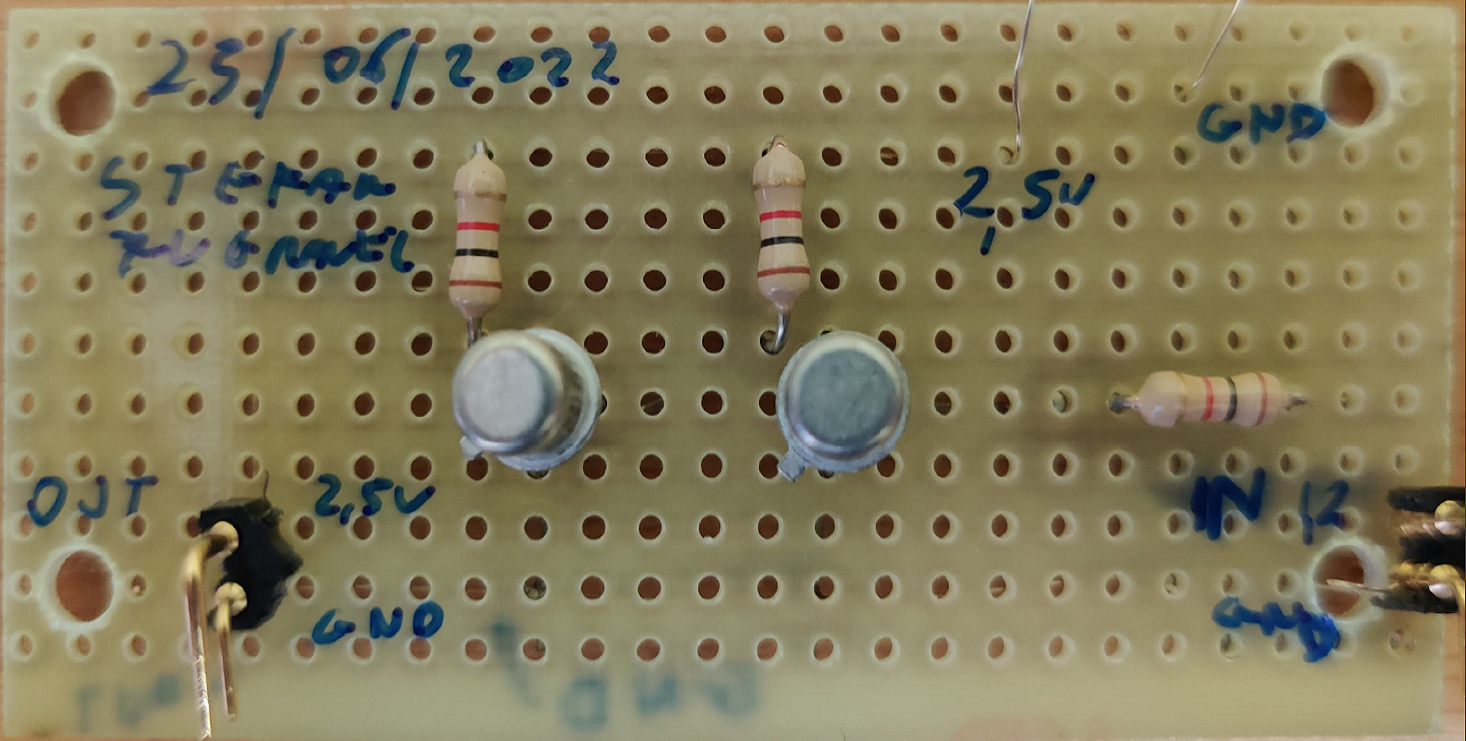
\includegraphics[width=.99\linewidth]{IMG/ch5/FRONTTRANSLATOR}
		\caption{Front view of the \\implemented translation device}
		\label{fig:fronttranslator}
	\end{minipage}%
	\begin{minipage}{.5\textwidth}
		\centering
		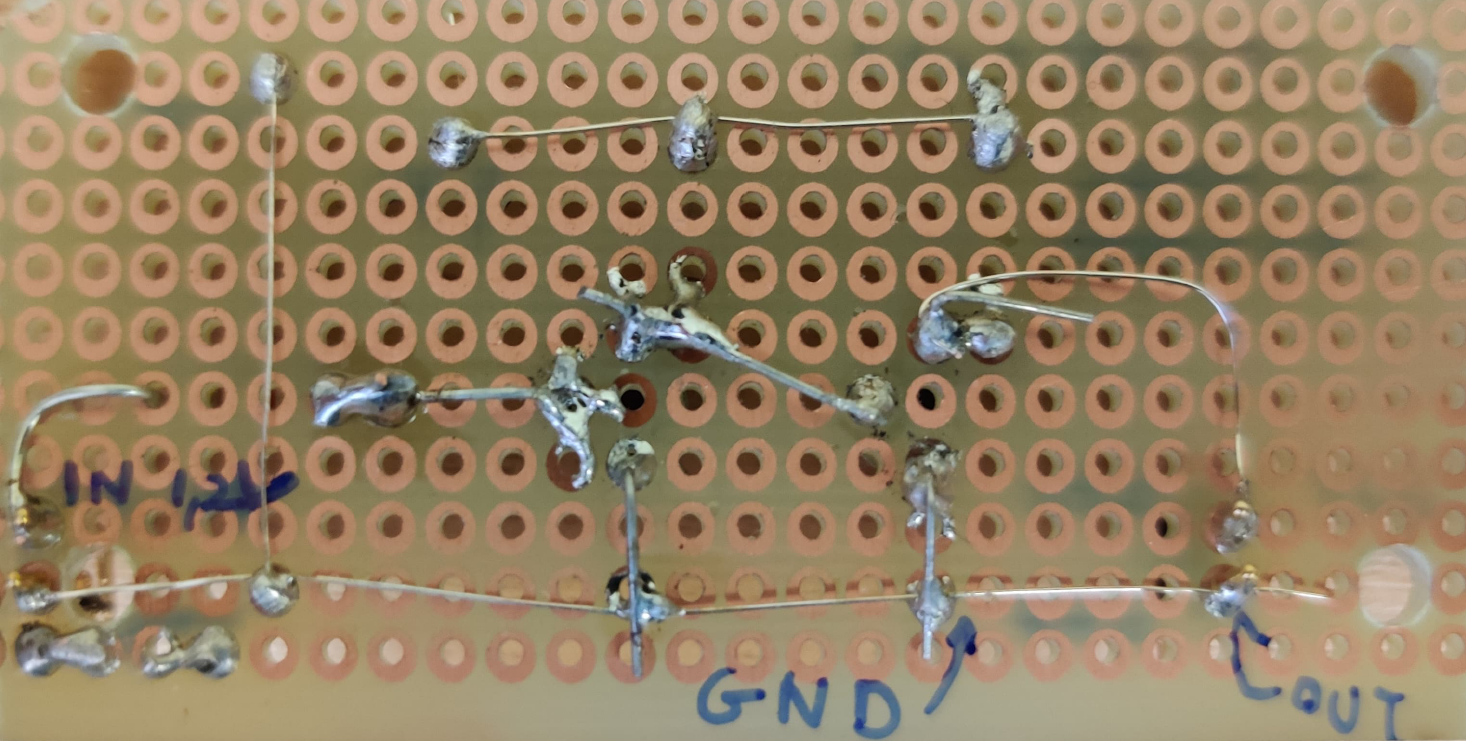
\includegraphics[width=.99\linewidth]{IMG/ch5/BACKTRANSLATOR}
		\caption{Back view of the \\implemented translation device}
		\label{fig:backtranslator}
	\end{minipage}
\end{figure}
\section{Firmware validation on board}

\subsection{Internal DACs test}\label{dactests}
%scrivi qualcosa del tipo: il processo di validazione è composto da due parti, una in cui l'oscilloscopio viene collegato direttamente alla board in modo da verificare il corretto output e una in cui la board viene collegata al chip
\noindent In order to validate the correct operation of
\begin{figure}[H]
	\centering
	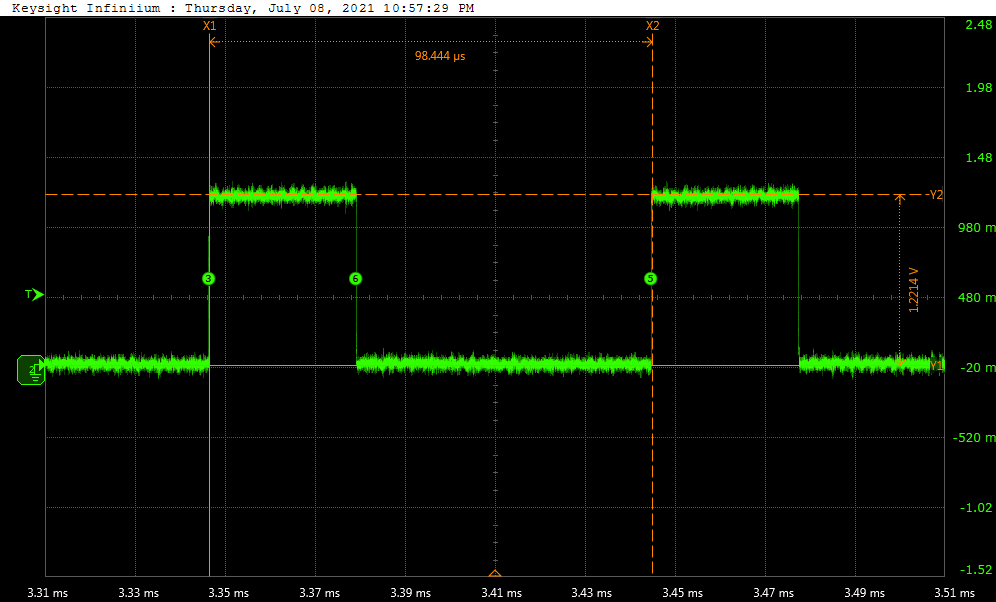
\includegraphics[width=0.7\linewidth]{IMG/ch5/probe/09-08-2021_clock-specks}
	\caption{}
	\label{fig:clockspecs}
\end{figure}

\subsubsection{Write command}
\begin{figure}[H]
	\centering
	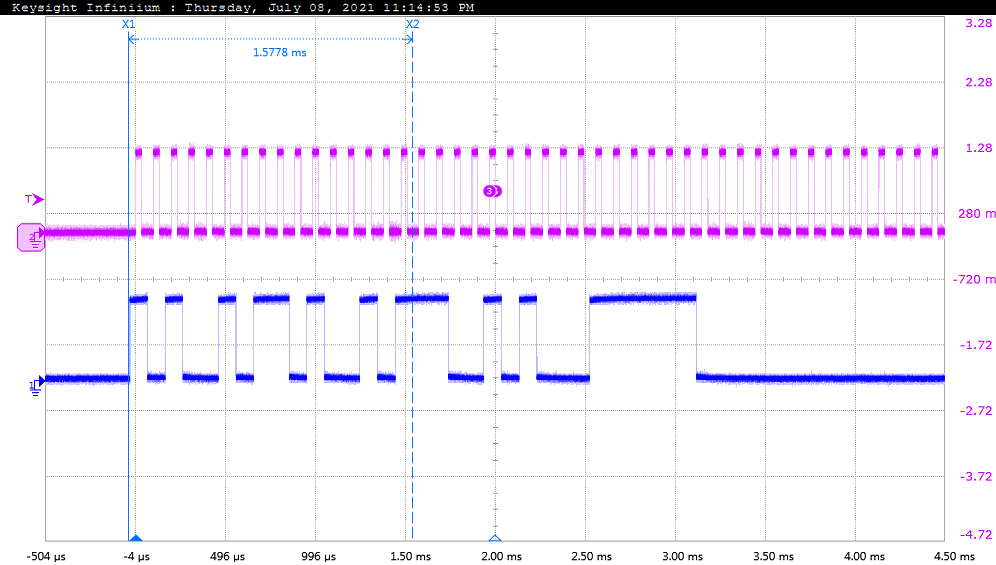
\includegraphics[width=0.7\linewidth]{IMG/ch5/probe/09-08-2021_ch05-write63-baselinedac1}
	\caption{}
	\label{fig:ch05write63}
\end{figure}

\subsubsection{Read command}
\begin{figure}[H]
	\centering
	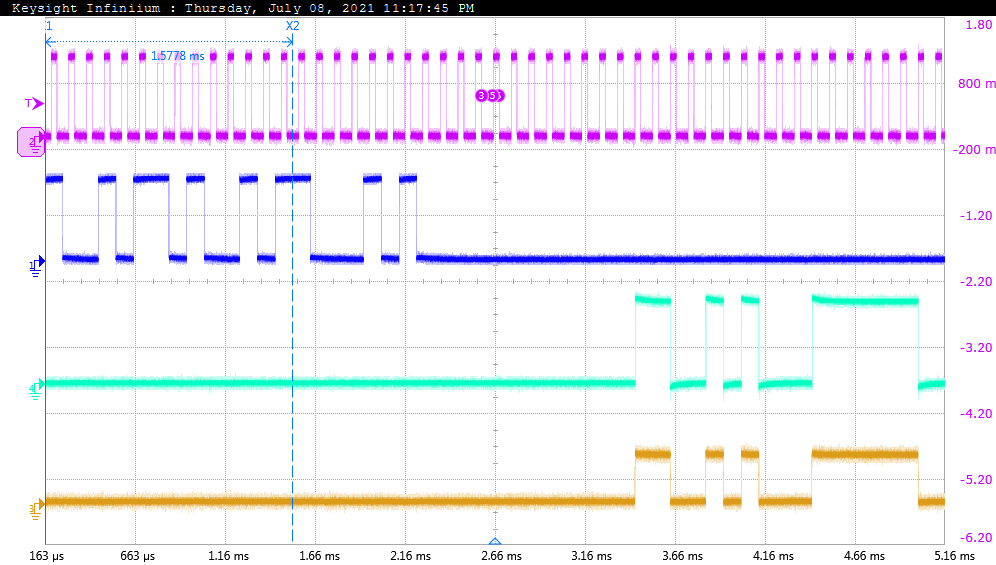
\includegraphics[width=0.7\linewidth]{IMG/ch5/probe/09-08-2021_ch05-read63-baselinedac1}
	\label{fig:ch05read63}
\end{figure}


\subsection{Latching counters test}

\subsection{Timestamp generator test}

\section{Esa-Abacus}